\section{Related Work}
\label{sec:related-work}

Our work sits at the intersection of several rapidly evolving research threads: the theoretical mechanics of in-context learning (ICL), implicit regularization in deep learning, and the kernel perspective on attention architectures. We position our contribution by tracing these lineages and highlighting the specific gap we address.

\subsection{Theoretical Mechanisms of In-Context Learning}
\label{subsec:theory-icl}

The quest to understand \textit{how} transformers learn from context began with analyses of simplified, linear models. The seminal insight, established concurrently by several groups, is that linear self-attention layers can implement gradient descent on a least-squares objective.

\begin{itemize}
	\item \textbf{Linear ICL as Gradient Descent.} \citet{von2023linear} provided a foundational mechanistic explanation, showing that a single linear self-attention layer can encode one step of gradient descent on a linear regression loss defined by the in-context examples. \citet{akyurek2022learning} arrived at a similar conclusion, demonstrating that transformers can implement learning algorithms for simple function classes. \citet{zhang2023trained} further analyzed the training dynamics, showing how gradient-based pre-training induces these algorithmic capabilities. The elegant conclusion from this line of work is that linear ICL is essentially implicit ridge regression, often corresponding to a minimum-norm solution.
	\item \textbf{Dynamical Systems View.} Building on this, \citet{giampaolo2023dynamical} and \citet{bai2024transformers} framed ICL as a dynamical system, analyzing the fixed points and stability of the transformer's forward pass when processing sequences of examples. This perspective connects ICL to iterative optimization algorithms beyond a single step.
\end{itemize}

\textbf{Limitation:} A critical and universal assumption in these works is the \textit{linearity} of the attention mechanism or the entire transformer block. While this simplification yields tractable and insightful theories, it surgically removes the very components—softmax and nonlinear activations—that define the transformer's expressive power. As a result, these theories are inherently limited to explaining ICL for \textit{linear} tasks and cannot characterize the behavior on nonlinear functions, which is the norm in practice.

\subsection{Implicit Regularization in Deep Learning}
\label{subsec:implicit-reg}

Implicit regularization refers to the tendency of gradient-based optimization to converge to solutions with desirable properties (e.g., simplicity, sparsity) without explicit penalties in the loss function.

\begin{itemize}
	\item \textbf{Linear Models \& Matrix Factorization.} For linear classifiers optimized with gradient descent, \citet{soudry2018implicit} and \citet{ji2020gradient} showed convergence to the max-margin (hard-margin SVM) solution. For matrix completion and factorization, \citet{gunasekar2017implicit, gunasekar2018characterizing} demonstrated implicit bias towards low-rank solutions. These works established that the optimization algorithm itself is a source of inductive bias.
	\item \textbf{Neural Tangent Kernel (NTK) Regime.} The NTK theory \citep{jacot2018neural, arora2019exact} revolutionized the analysis of over-parameterized neural networks. It shows that in the infinite-width limit, training a network with gradient descent is equivalent to kernel regression with a deterministic kernel—the NTK. This provides a powerful tool to derive generalization bounds \citep{cao2019generalization}. Our work leverages the NTK formalism to analyze the MLP component of the transformer.
	\item \textbf{Beyond NTK: Feature Learning.} Recent efforts focus on the \textit{finite-width} regime where feature learning occurs \citep{woodworth2020kernel, yang2021tensor}. While highly relevant, the analysis becomes significantly more complex. Our current work adopts the NTK perspective for the MLP to obtain tractable, first-order theoretical results, acknowledging this as a starting point for future exploration into feature learning within ICL.
\end{itemize}

\textbf{Crucial Distinction:} The aforementioned literature almost exclusively analyzes a \textit{fixed} dataset drawn from a \textit{single} task distribution. The learning problem is: given dataset $\mathcal{D}$, find parameters $\theta$ that minimize $\mathcal{L}(\theta; \mathcal{D})$. In stark contrast, ICL is a \textit{meta-learning} scenario. The model is pre-trained on a distribution of tasks $\mathcal{P}(\mathcal{T})$. At test time, it is presented with a new, small dataset $\mathcal{D}_{\text{context}}$ from a new task $\mathcal{T}_{\text{new}} \sim \mathcal{P}$, and must make a prediction. The object of implicit regularization is therefore not a single function $f_\theta$, but the \textit{learning algorithm} $A_\theta$ that maps $\mathcal{D}_{\text{context}}$ to a prediction function. This fundamental difference necessitates a novel theoretical framework.

\subsection{Attention, Kernel Methods, and Representation Learning}
\label{subsec:attention-kernel}

The connection between attention mechanisms and kernel methods provides a vital mathematical language for our analysis.

\begin{itemize}
	\item \textbf{Attention as Kernel Smoothing.} Early works by \citet{tsai2019transformer} and \citet{katharopoulos2020transformers} reinterpreted attention weights as kernel values, drawing parallels to Nadaraya-Watson kernel regression. This view frames the attention output as a weighted average of values, where weights are determined by a similarity kernel between queries and keys.
	\item \textbf{Kernel Perspective on ICL.} This idea was extended specifically to ICL by \citet{chen2024kernels} and contemporaneous work. They showed that softmax attention defines an implicit feature map, and transformer-based ICL can be seen as performing kernel gradient descent in that feature space. This was a significant step towards a nonlinear theory.
	\item \textbf{Mechanistic Interpretability.} Complementary work in mechanistic interpretability seeks to reverse-engineer the algorithms learned by transformers. Studies on induction heads \citep{elhage2021mathematical} and task vectors \citep{ilharco2022patching} reveal that transformers can implement primitive operations like copying and pattern matching. This line of research provides empirical evidence for the \textit{existence} of learned algorithms, which our work aims to characterize statistically.
\end{itemize}

\textbf{Our Synthesis:} Prior kernel-based analyses of ICL often focused on the attention mechanism in isolation or in linearized settings. They did not fully integrate the \textit{nonlinear Multi-Layer Perceptron (MLP)}, a core component that contributes the bulk of parameters and nonlinear expressive power in standard transformers \citep{sohn2024understanding}. Our work unifies these threads: we treat the \textit{full transformer block} (self-attention + nonlinear MLP) as a composite system that induces a \textit{structured, combined kernel} ($K_{\text{att}} + K_{\text{mlp}}$). This allows us to analyze the implicit regularization of the complete architecture.

\subsection{Early Explorations of Nonlinearity in ICL}
\label{subsec:nonlinear-explore}

The community has recently begun to grapple with the necessity and role of nonlinearity in ICL.

\begin{itemize}
	\item \textbf{Empirical Necessity.} \citet{sohn2024understanding} conducted careful ablation studies, showing that transformers with linearized attention or MLPs fail catastrophically at nonlinear ICL tasks, while standard transformers succeed. This empirically underscores that nonlinearity is not a minor detail but a fundamental requirement.
	\item \textbf{Theoretical Steps.} \citet{liu2023theoretical} provided an initial analysis of shallow ReLU networks in a meta-learning setup akin to ICL, deriving generalization bounds. While insightful, their model does not incorporate the attention mechanism, which is the defining feature of the transformer architecture and crucial for processing variable-length context.
\end{itemize}

\textbf{The Open Problem:} Despite these important steps, a \textit{unified, end-to-end theoretical analysis} of the implicit regularization and generalization properties of a standard transformer (with softmax attention \textit{and} nonlinear MLP) performing ICL has been missing. Existing work either linearizes the architecture, removes key components, or does not provide finite-sample generalization guarantees grounded in the architecture's parameters.

\subsection{Our Position in the Landscape}

We summarize the relationship of our work to the existing literature in \cref{fig:landscape}.

% \begin{figure}[htbp]
% 	\centering
% 	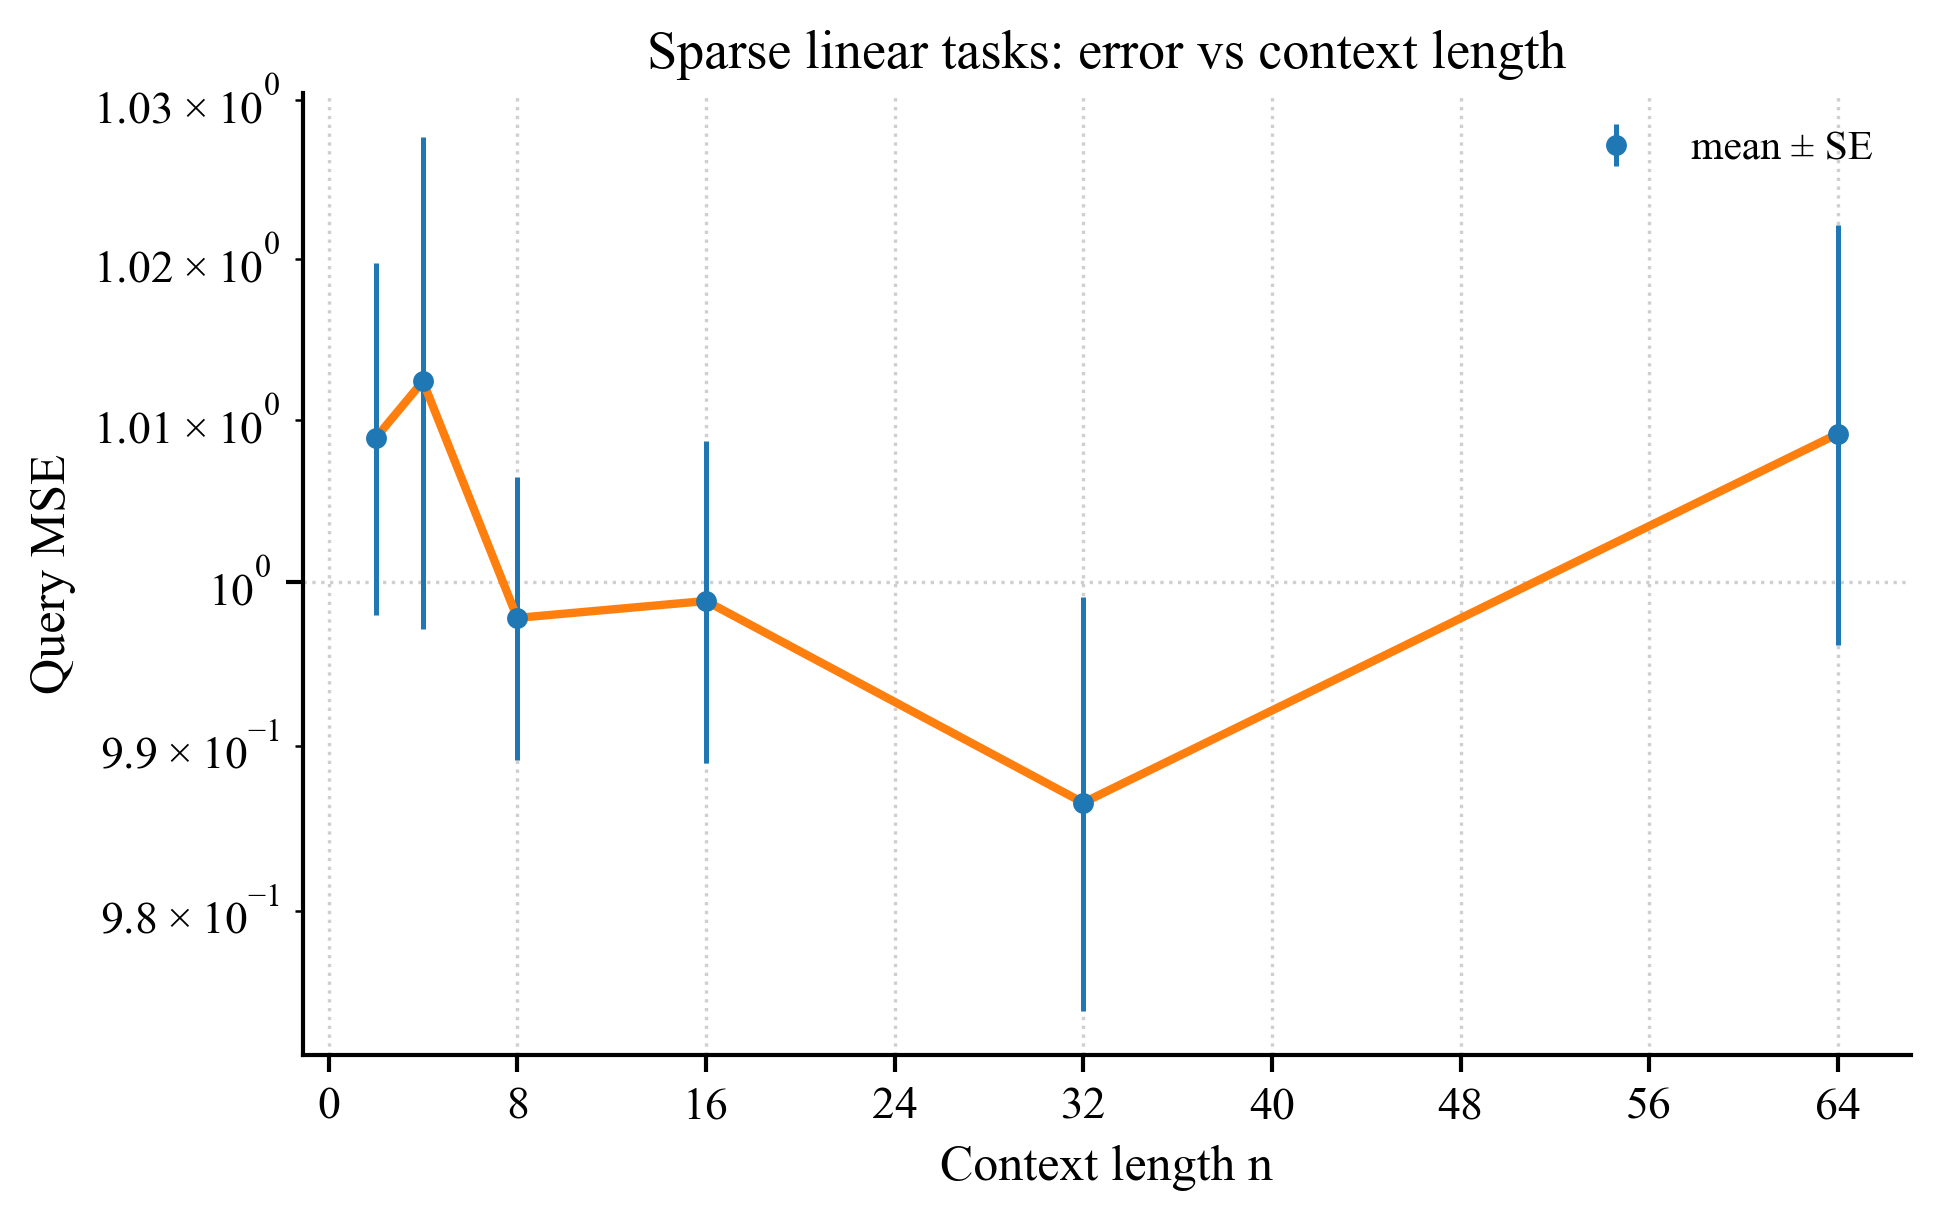
\includegraphics[width=0.5\linewidth]{figures/placeholder.png} % Assume this figure is generated
% 	\caption{Theoretical landscape of ICL. Existing linear theories analyze simplified models (left). Kernel methods connect attention to kernels but often neglect the MLP or nonlinearity (middle). Our work provides a unified analysis of the full, nonlinear transformer block, deriving its implicit regularization as kernel ridge regression with a structured kernel and discovering a phase transition in its behavior.}
% 	\label{fig:landscape}
% \end{figure}
\textbf{Figure Description:} A three-panel diagram. Panel 1 (Left): Labeled "Linear ICL Theories," showing a simplified transformer diagram with "Linear Attention" and "No MLP," pointing to equations for gradient descent/ridge regression. Panel 2 (Middle): Labeled "Kernel Perspectives," showing a transformer with "Softmax Attention" connected to a kernel $K_{\text{att}}$, but the MLP is grayed out or labeled "Linear/Approximated." Panel 3 (Right): Labeled "This Work," showing a complete transformer block with both "Softmax Attention" and "Nonlinear MLP (ReLU)," converging to a combined kernel $K_{\text{total}} = \alpha K_{\text{att}} + \beta K_{\text{mlp}}$ and a phase transition curve for the regularization behavior.

In short, this paper bridges the gap between the elegant but limited linear ICL theories and the complex reality of nonlinear transformers. We achieve this by developing a novel theoretical framework that treats the transformer as a kernel machine in a carefully constructed RKHS, enabling us to derive the first finite-sample generalization bounds for nonlinear ICL and uncover its dynamic regularization behavior.
